\documentclass[a4paper,10pt]{article}

%% Paquetes Adicionales %%

\usepackage[spanish]{babel}
\selectlanguage{spanish}
\spanishdecimal{.}
\addto\captionsspanish{\def\tablename{Cuadro}}
\usepackage{fancyhdr}
\usepackage{graphics}
\usepackage[dvips]{graphicx}
\usepackage[normal]{caption2}
\usepackage{amsfonts,amssymb,amsmath,amsthm}
\usepackage[T1]{fontenc}
\usepackage{moreverb}

%% Declaracion de comandos %%

\newtheorem{lema}{Lema}
\newtheorem{teor}{Teorema}
\newtheorem{propos}{Proposici\'on}
\newtheorem{corol}{Corolario}

\newcommand{\mivec}[1]{\mathbf{#1}}
\newcommand{\vers}[1]{\mivec{\check{#1}}}
\newcommand{\deriv}[2]{\frac{\mathrm{d}#1}{\mathrm{d}#2}}
\newcommand{\expo}[1]{~10^{#1}}
\newcommand{\uni}[1]{\mathrm{#1}} 

\newcommand{\prop}[1]{\begin{propos} #1 \end{propos}}
\newcommand{\teo}[1]{\begin{teor} #1 \end{teor}}
\newcommand{\cor}[1]{\begin{corol} #1 \end{corol}}
\newcommand{\lem}[1]{\begin{lema} #1 \end{lema}}

%% Encabezado y Pie de Pagina %%

\pagestyle{plain}
\lhead{}
\chead{}
\rhead{}
\cfoot{\thepage}
\renewcommand{\footrulewidth}{0.4pt}

%%\author{Juan Ignacio Go\~ni}

\makeindex

%% Titulo %%
\begin{document}
\title{{\ Trabajo pr\'actico final \\ Robot recolector de residuos \\ Placa m\'odulo gen\'erico}}

%\date{}

%% Comienzo del documento %%

\maketitle

\begin{abstract}
En el presente se establecen las especificaciones para la placa del m\'odulo gen\'erico.
Se expone el circuito de la placa, explica funcionamiento y se muestran posibles usos.

\textbf{Palabras Clave: }\emph{Robot, residuos, protocolo, serial, rs-232, daisy chain}.
\end{abstract}

%\thispagestyle{fancy}

%% COMIENZO DEL TEXTO %%

\section{Introducci\'on}
\label{introduccion}

**TODO**

\section{Microcontrolador}
\label{microcontrolado}

El microcontrolador elegido para la placa es el 16F88 de Microchip.
Cuenta con una memoria \emph{FLASH} para 4096 instrucciones de programa, una memoria \emph{RAM} de 368 bytes y una memoria \emph{EEPROM} de 256 bytes.
En la subsecci\'on \ref{perifericos} se listan algunos de los principales perif\'ericos incluidos en el microcontrolador.
Se utiliza con un cristal externo de 20MHz como clock.

Para la carga y debug del firmware espec\'ifico para cada placa se utiliza el programador \emph{ICD2}, como se explica en la secci\'on \ref{programador}.
Cuenta con un reducido set de instrucciones b\'asicas todas con el mismo tiempo de ejecuci\'on.

\subsection{Perif\'ericos}
\label{perifericos}

El microcontrolador 16F88 cuenta con 2 puertos de 8 entradas y salidas cada uno de tipo TTL y CMOS.
Cada pin se encuentra multiplexado con uno o m\'as perif\'ericos internos.

\subsubsection{Timers}
\label{timers}

Cuenta con 3 timers o contadores.

El \emph{TMR0} es de 8 bits y contiene un \emph{preescaler} de 8bits, es usado como WDT.
Tambi\'en puede ser utilizado como contador externo por el pin \emph{RA4}.

El \emph{TMR1} es de 16 bits y contiene un \emph{preescaler} de 2bits.
Puede ser utilizado como contador externo por el pin \emph{RB6} o con un cristal externo conectado a los pines \emph{RB6} y \emph{RB7}.

El \emph{TMR2} es de 8 bits, contiene un \emph{preescaler} de 2 bits y contiene un \emph{postscaler} de 4 bits.
Es de vital importancia para el m\'odulo de PWM por hardware.

\subsubsection{ADC}
\label{adc}

Cuenta con un conversor anal\'ogico digital de 8 o 10 bits multiplexado en 7 canales, 5 canales en el puerto A y 2 en el puerto B.
Es posible definir voltajes de referencia mediante ciertos pines o usar valores internos de referencia como \emph{Vcc} y \emph{GND}.

\subsubsection{PWM}
\label{pwm}

Cuenta con un m\'odulo de generaci\'on de un PWM por hardware de 10 bits de resoluci\'on con el ciclo y per\'iodo configurable mediante el \emph{TMR2}

\subsubsection{AUSART}
\label{ausart}

Cuenta con un m\'odulo de UART para comunicaci\'ion sincr\'onica o asincr\'onica utilizado para la implementaci\'on del daisy chain por RS-232.

\subsubsection{Otros}
\label{otros}

Para mayor informaci\'on respecto a los perif\'ericos o configuraci\'on del microcontrolador, se recomienda revisar las hojas de datos directo del fabricante.

\section{Comunicaci\'on}
\label{comunicacion}
 
El protocolo de comuncaci\'on consta de paquetes que son enviados con un destinatario espec\'ifico
y representa un pedido de informaci\'on o comando que debe ser ejecutado en destino.

Ver la documentaci\'on del protocolo para mayor informaci\'on.

La comunicaci\'on est\'a basada en el m\'etodo \emph{Daisy chain} (patente US20090316836A1).
La cadena se construye con las placas controladoras, las cuales se comunican entre ellas retransmitiendo cada paquete hacia adenlante.

\begin{figure}
\centering
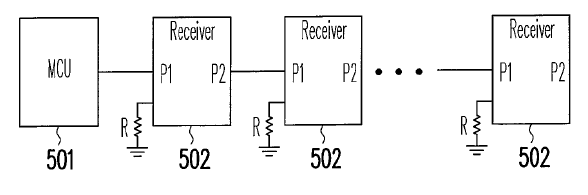
\includegraphics[scale=0.75]{daisychain_diagram.png}
\caption{Diagrama general del m\'etodo daisy chain}
\label{daisychain_diagram}
\end{figure}

La mayoria de los paquetes o mensajes enviados se originan en el controlador principal que luego recibe una respuesta de confirmaci\'on de recepci\'on.

Como parte de la configuraci\'on de la placa, existe un switch que determina el tipo de ***eslavon*** de la placa, si es un nodo intermedio
o la punta de la cadena.

En la figura \ref{daisychain_pinout} se especifica el pinout del puerto de entrada y de salida.
Tambi\'en se especifica el conexionado contra el controlador principal.

\begin{figure}
\centering
\includegraphics[scale=1]{daisychain_pinout.png}
\caption{Pinout de los puertos de comuncaci\'ion de entrada y salida}
\label{daisychain_pinout}
\end{figure}

\section{Alimentaci\'on}
\label{alimentacion}

La alimentaci\'on principal de la placa es 7 a 20 voltios, con la posibilidad de alimentarla directamente 
con 5 voltios por uno de los pines del conector, ver figura \ref{alimentacion_pinout}.

\begin{figure}
\centering
\includegraphics[scale=1]{alimentacion_pinout.png}
\caption{Pinout de la alimentaci\'on de la placa}
\label{alimentacion_pinout}
\end{figure}

\section{Configuraci\'on}
\label{configuracion}

switches, headers de leds y pines

\section{Posibles usos}
\label{usos}

uso de los pines...

\section{Esquem\'atido}
\label{esquematico}

esquematico de la placa

\section{Circuito}
\label{circuito}

capas del circuito

\section{El programador}
\label{programador}

pines de conexionado, modelo, marca, bla

\section{C\'odigo b\'asico}
\label{codigo}

codigo minimo para que funcione con el protocolo, includes, etc...

\end{document}